\section{Zabezpieczenie Infrastruktury Teleinformatycznej:}
\subsection{Cel i Istota Zabezpieczenia}

Zastosowanie Zasilacza Bezprzerwowego (UPS, Uninterruptible Power Supply) ma na celu zapewnienie ciągłości zasilania w sytuacjach awaryjnych lub niestabilnych warunkach zasilania. Oto kilka kluczowych celów i istotnych aspektów związanych z zabezpieczaniem systemów za pomocą UPS:


\begin{enumerate}
    \item Zapewnienie Ciągłości Działania
        \begin{itemize}
            \item Głównym celem UPS jest utrzymanie zasilania urządzeń elektrycznych, takich jak komputery, serwery, sprzęt sieciowy itp., w przypadku utraty zasilania głównej sieci energetycznej.
        \end{itemize}


    \item Ochrona przed Skokami Napięcia i Spadkami Napięcia
        \begin{itemize}
            \item UPS chroni podłączone urządzenia przed szkodliwymi skokami i spadkami napięcia, co może uszkodzić sprzęt elektroniczny.
        \end{itemize}

    \item Zabezpieczenie przed Przerwami w Zasilaniu
        \begin{itemize}
            \item UPS umożliwia pracę na sprzęcie przez pewien czas po utracie zasilania, co pozwala na bezpieczne zamknięcie systemu operacyjnego lub zapisanie danych przed całkowitym wyłączeniem urządzeń.
        \end{itemize}

    \item Ochrona Przed Awariami Zasilania
        \begin{itemize}
            \item W przypadku awarii zasilania, UPS działa jako źródło awaryjne, co pomaga uniknąć przerw w pracy systemów krytycznych dla firm.
        \end{itemize}
    
    \item Zminimalizowanie Ryzyka Utraty Danych
        \begin{itemize}
            \item UPS daje użytkownikom wystarczająco dużo czasu, aby zapisać i zamknąć dane, co pomaga w zminimalizowaniu ryzyka utraty danych w przypadku nieoczekiwanej utraty zasilania
        \end{itemize}
    
    \item Ochrona Przed Skutkami Przepięć Błyskawicznych
        \begin{itemize}
            \item Niektóre UPS posiadają funkcje filtracji przeciwprzepięciowej, które chronią podłączone urządzenia przed skutkami przepięć, w tym tych wywołanych uderzeniem pioruna.
        \end{itemize}

    
    \item Zwiększenie Łącznej Stabilności Systemu
    \begin{itemize}
        \item Korzystanie z UPS wpływa na ogólną stabilność systemu, zwłaszcza w miejscach, gdzie występują niestabilne warunki zasilania.
    \end{itemize}
    
    \item Podtrzymanie Zasilania w Krytycznych Aplikacjach
    \begin{itemize}
        \item W przypadku systemów krytycznych, takich jak szpitale, laboratoria czy centra przetwarzania danych, UPS jest kluczowym elementem zapewniającym ciągłość działania.
    \end{itemize}
\end{enumerate}

\pagebreak

\subsection{Wybór Mocy Zabezpieczenia 15 kW i Czas Pracy w Trybie Awaryjnym (48 godzin)}


Wstawiając dane pod wzór: 
\begin{align*}
    E & = \text{Łączna energia (kWh)} \\
    P & = \text{Moc jednego UPS (kW)} \\
    \text{Liczba UPS} & = \frac{E}{P} \\
    \text{Liczba UPS} & = \frac{864 \, \text{kWh}}{15 \, \text{kW}} \approx 57.6
\end{align*}


\subsection{Specyfikacja Techniczna Sprzętu Awaryjnego}
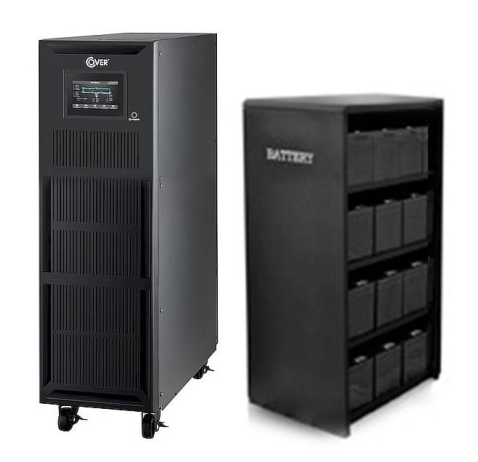
\includegraphics[width=0.3\textwidth]{1-szafa.png}
\begin{itemize}
    \item Moc pozorna / Moc czynna : 15000VA (15000W)
    \item Rodzaj UPS: Online 3-Fazowy 3/1, 3/3
    \item Technologia: TRUE ON-LINE Double Conversion (prawdziwa podwójna konwersja)
    \item Power Factor wyjściowy: 1.0
    \item Rodzaj obudowy: Tower
    \item Wyjście / wyjście: TERMINAL (zaciski śrubowe)
    \item Ilość oraz rodzaj baterii: zew. moduł bateryjny C10 (36x18Ah)
    \item Czas podtrzymania: 15 minut (przy obciążeniu 100%)
    \item Porty komunikacyjne: USB, EMBS, złącza pracy równoległej
    \item Zerowy czas przełączania w tryb awaryjny
    \item Wyłącznik EPO umożliwia natychmiastowe odłączenie zasilania od odbiorników
    \item Wyłącznik REPO umożliwia zdalne odłączenie zasilania odbiorników w przypadku pożaru
    \item Panel kontrolno-monitorujący LCD oraz wskaźnik LED
    \item Złącze dla zewnętrznego modułu bateryjnego
    \item Inteligentny Slot na moduł rozszerzeń (np. SNMP do kontroli zdalnej)
    \item opcjonalnie: moduł SNMP, ModBus, DryContact, RS232, RS485
    \item Zabezpieczenia:  przeciwprzepięciowe, przeciwzwarciowe, przeciwprzeciążeniowe, ochrona przed prądem wstecznym
    \item Wymiary UPS: 250 x 827 x 627mm (szer. x wys. x gł.)
    \item Wymiary MB: 880 x 1190 x 950mm (szer. x wys. x gł.)
    \item Oprogramowanie: ViewPower
\end{itemize}


\subsection{Schemat Logiczny Podłączenia}
    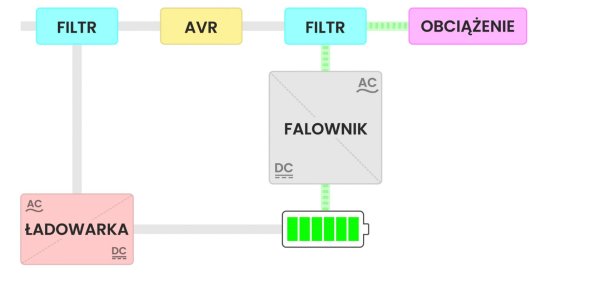
\includegraphics[width=0.8\textwidth]{2-schemat.png}

    

\subsection{Kosztorys Zabezpieczenia Infrastruktury}
\begin{flushleft}
    \begin{table}[h]
        \renewcommand{\arraystretch}{1.5}
        \begin{tabular}{|l|l|r|r|}
            \hline
            \textbf{Nazwa} & \textbf{Szt.} & \textbf{Cena [zł]} & \textbf{Wartość [zł]} \\
            \hline
            Zasilacz awaryjny UPS 3-fazowy 15kVA/15kW 3:3 & 58 & 20 973,06 & 1 216 437,48 \\
            \hline
        \end{tabular}
    \end{table}
\end{flushleft}
